\chapter{Base de dados documental - MongoDB}
\paragraph{}
Para armazenar os nossos dados numa base de dados não relacional e orientada a documentos, recorremos ao \textbf{MongoDB}. Inicialmente, dedicamos bastante tempo à avaliação do esquema da base de dados relacional existente para decidir a melhor forma de representar os dados na nova estrutura orientada a documentos, aproveitando ao máximo as vantagens deste paradigma. Com base nesta análise e considerando as consultas futuras que serão realizadas, decidimos dividir a base de dados em três coleções principais:

\begin{enumerate}
    \item \textbf{Pacientes:} Armazena informações sobre os pacientes, os seus contactos de emergência, histórico médico e informações do seguro.
    \item \textbf{Staff:} Inclui dados sobre médicos, enfermeiros e técnicos, juntamente com as suas respetivas informações do departamento onde trabalham.
    \item \textbf{Episódios:} Contém detalhes sobre os episódios de atendimento médico, incluindo consultas, hospitalizações, prescrições, faturas e exames laboratoriais.
\end{enumerate}

Para a migração dos dados de Oracle para MongoDB utilizou-se o script \mintinline{python}{migrate_to_mongo.py} que efetua uma conexão com a base de dados Oracle, de forma a permitir a recolha dos dados. Após a obtenção dos dados da base de dados relacional, realizamos o devido tratamento e criação das coleções acima propostas e que serão abordadas nos capítulos seguintes. Para finalizar, realizamos uma segunda conexão, agora à base de dados MongoDB e carregamos as coleções resultantes para esta base de dados não relacional. 

Este script foi criado para facilitar a implementação dos dados em MongoDB de forma a que seja possível uma transferência eficiente e estruturada dos dados sempre que necessário.

\begin{figure}[H]
    \centering
    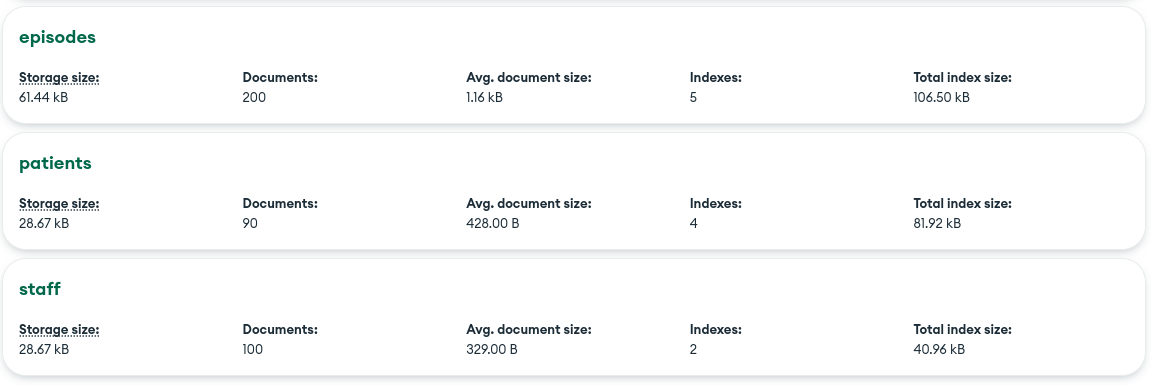
\includegraphics[width=0.9\linewidth]{Imagens/MongoDB/colecoes_mongo.png}
    \caption{Coleções criadas na base de dados MongoDB}
    \label{fig:colecoes_mongo}
\end{figure}

\section{Coleção Pacientes}
A coleção de Pacientes no MongoDB foi projetada para armazenar informações abrangentes sobre cada paciente, aproveitando a flexibilidade da estrutura de documentos JSON. Esta coleção inclui dados pessoais como nome, data de nascimento, tipo sanguíneo, contacto telefónico e e-mail. Além disso, armazena detalhes de seguros de saúde, contactos de emergência e histórico médico. No final um objeto paciente pertencente a esta coleção terá uma estrutura semelhante à seguinte:

\begin{myminted}{json}
{
  "_id": {"|\$|oid": "6658a65bf6d1a33ea5c68337"},
  "id_patient": 2,
  "patient_fname": "Jane",
  "patient_lname": "Smith",
  "blood_type": "O-",
  "phone": "987-654-3210",
  "email": "jane.smith@example.com",
  "gender": "Female",
  "birthday": {"|\$|date": "1990-03-20T00:00:00.000Z"},
  "insurance": {
    "policy_number": "POL002",
    "provider": "XYZ Insurance",
    "insurance_plan": "Premium Plan",
    "co_pay": 30,
    "coverage": "Partial Coverage",
    "maternity": false,
    "dental": true,
    "optical": true
  },
  "emergency_contact": [
    {
      "contact_name": "Jane Smith",
      "phone": "222-333-4444",
      "relation": "Mother"
    }
  ],
  "medical_history": [
    {
      "record_id": 2,
      "condition": "Allergy",
      "record_date": {"|\$|date": "2023-03-05T00:00:00.000Z"}
    }
  ]
}
\end{myminted}


\section{Coleção Staff}
A coleção de Staff no MongoDB foi desenvolvida para gerir de forma eficiente os dados relacionados aos funcionários do sistema de saúde, incluindo médicos, enfermeiros e técnicos. Esta coleção armazena informações detalhadas sobre cada funcionário, como nome, data de admissão, endereço, e-mail e número de segurança social. Também inclui detalhes específicos sobre o departamento ao qual pertencem, suas qualificações e o estado de atividade atual. Na base esta coleção faz uso da semelhança entre as tabelas de \textit{doctor}, \textit{nurse} e \textit{technician} agrupando-as com a tabela \textit{staff} e \textit{department}, utilizando o campo \textit{\textbf{role}} para identificação do funcionário de saúde em questão (\textit{DOCTOR}, \textit{NURSE}, \textit{TECHNICIAN}). O atributo \textit{\textbf{date\_of\_separation}} apenas se encontra presente nos funcionários que já abandonaram um determinado departamento, quando tal não acontece este campo não é acrescentado ao objeto JSON. Em seguida é apresentado um exemplo da estrutura implementada para o caso de um médico que ainda se mantém ativo no departamento em questão:

\begin{myminted}{json}
{
  "_id": {"|\$|oid": "6658a65bf6d1a33ea5c6838a"},
  "emp_id": 6,
  "emp_fname": "Lisa",
  "emp_lname": "Hayes",
  "date_joining": {"|\$|date": "2023-05-10T00:00:00.000Z"},
  "email": "mprice@example.com",
  "address": "Trevorfurt, IN 02637\"",
  "ssn": 685569160,
  "is_active_status": true,
  "department": {
    "id_department": 1,
    "department_head": "John Smith",
    "department_name": "Cardiology_1"
  },
  "role": "DOCTOR",
  "qualifications": "PhD"
}
\end{myminted}

\section{Coleção Episódios}

A coleção de Episódios no MongoDB foi criada para armazenar informações detalhadas sobre os episódios de atendimento dos pacientes, incluindo consultas, hospitalizações, prescrições, faturas e exames laboratoriais. Como esta coleção serve como uma ligação essencial entre as coleções de Pacientes e Staff, foi necessário encontrar uma maneira eficiente de traduzir essas relações. Uma das abordagens consideradas foi a criação de redundância nas coleções, aproveitando a flexibilidade do paradigma não relacional para replicar dados e adicionar informações úteis diretamente na coleção de Episódios. No entanto, para evitar a redundância excessiva, optou-se por utilizar identificadores de objetos de outras coleções, funcionando de maneira similar às chaves estrangeiras no paradigma relacional. Esta abordagem permite manter a integridade referencial e facilita consultas mais eficientes e organizadas, garantindo, assim, uma gestão mais eficaz dos dados. 

Para implementar esta abordagem, foi necessário armazenar em duas listas os IDs dos objetos de Pacientes e Staff que foram adicionados. Em Python, essa tarefa foi facilitada pelo uso da função \mintinline{python}{collection.insert_many()}. Esta função não apenas insere os elementos na coleção correspondente, mas também retorna um objeto contendo a lista de todos os IDs inseridos. Assim, antes de migrar os dados para a coleção de episódios, bastou obter duas listas contendo todos os IDs dos pacientes e membros do staff previamente inseridos. Com estas listas carregadas, foi possível estabelecer as relações necessárias entre as coleções de forma eficiente e precisa, garantindo que, por exemplo, cada episódio estivesse corretamente associado aos seus respetivos paciente e profissional de saúde. Se um indivíduo desta coleção fosse hospitalizado, recebesse prescrições de medicamentos e fosse submetido a exames médicos, a sua estrutura seria representada da seguinte forma na coleção:

\begin{myminted}{json}
{
  "_id": {"|\$|oid": "66603d8cc0c3dd4601195502"},
  "id_episode": 175,
  "id_patient": {"|\$|oid": "66603d8cc0c3dd460119543d"},
  "hospitalization": {
    "admission_date": {"|\$|date": "2020-11-03T00:00:00.000Z"},
    "discharge_date": {"|\$|date": "2020-11-04T00:00:00.000Z"},
    "responsible_nurse": {"|\$|oid": "66603d8cc0c3dd46011954ca"},
    "room": {
      "id_room": 40,
      "room_type": "Executive",
      "room_cost": 420
    }
  },
  "prescriptions": [
    {
      "id_prescription": 169,
      "prescription_date": {"|\$|date": "2020-11-03T00:00:00.000Z"},
      "dosage": 31,
      "medicine": {
        "id_medicine": 1,
        "m_name": "Paracetamol",
        "m_quantity": 50,
        "m_cost": 10
      }
    }
  ],
  "lab_screenings": [
    {
      "lab_id": 9,
      "test_cost": 93.19,
      "test_date": {"|\$|date": "2020-11-03T00:00:00.000Z"},
      "id_technician": {"|\$|oid": "66603d8cc0c3dd46011954f6"}
    }
  ]
}

\end{myminted}



\section{Triggers em MongoDB}
Durante o processo de migração de dados da base de dados Oracle para MongoDB, foi necessário definir diversos \textit{triggers} para otimizar a inserção de novos documentos e manter a integridade dos dados. Na nossa base de dados, procurávamos evitar o uso manual de campos de identificação durante a inserção de novos documentos preservando os campos de identificação originais, provenientes da base de dados Oracle, e mantendo a utilização de campos de identificação do mesmo tipo na base de dados MongoDB (além da utilização de identificadores do tipo ObjectId para o campo '\_id'). Para tal, utilizamos \textit{triggers} responsáveis por gerar automaticamente esses identificadores, garantindo a integridade e a unicidade dos dados.

Para alcançar este objetivo, optamos pela criação de uma coleção auxiliar denominada '\textit{counters}', responsável por armazenar o valor máximo de cada identificador inteiro existente, entre todos os valores já utilizados até ao momento. Cada documento desta coleção é utilizado para a geração do próximo valor de cada identificador único (similar às sequências em Oracle) durante a inserção de novos documentos ou substituição de documentos existentes nas restantes coleções da base de dados. Assim, na inserção de um novo documento, o contador correspondente, presente neste coleção '\textit{counters}', é incrementado, de modo obter o próximo valor do identificador, de acordo com a coleção na qual foi inserido um novo documento e o identificador em questão.

Além dos \textit{triggers} relacionados à criação de identificadores únicos, foi necessário adaptar um \textit{trigger} existente na base de dados original Oracle para o ambiente MongoDB. Este \textit{trigger} específico foi ajustado para garantir que sua funcionalidade fosse preservada após a migração, mantendo a consistência e a continuidade das operações automatizadas.

Em MongoDB, para a configuração e \textit{deployment} destes triggers, decidimos utilizar um \textit{cluster} criado na plataforma \textit{MongoDB Atlas}. Assim, de modo a automatizar a criação de triggers nesta plataforma, desenvolvemos diversos \textit{scripts} Python responsáveis pela criação, atualização, remoção e retoma (após uma falha no cluster, por exemplo) dos triggers na mesma, que utilizam pedidos \textit{HTTP} a APIs disponibilizadas pelo MongoDB de modo a efetuar as diversas operações descritas.


\subsection{Triggers para a adição de identificadores únicos}
Na sequencia da criação destes \textit{triggers} foi observada a existência de dois casos de geração de identificadores diferentes. Estes dois casos distintos dividiram a implementação em dois tipos principais: \textit{triggers} responsáveis pela geração de valores para os identificadores de cada documento e, \textit{triggers} responsáveis pela geração de valores para identificadores de objetos armazenados em listas/arrays presentes nos documentos das restantes coleções.

Assim sendo, para os campos 'id\_patient', 'id\_episode' e 'emp\_id', das coleções 'patients', 'episodes' e 'staff, respetivamente, foram criados três \textit{triggers} idênticos, acionados sempre que seja necessário gerar um novo identificador como valor de algum destes três campos, ou, caso o utilizador decida especificar o valor do identificador manualmente e possa, eventualmente, ser necessário atualizar o valor do contador correspondente ao campo em questão, para o valor do identificador inserido manualmente (caso este seja superior ao valor do contador). Deste modo, estes \textit{triggers} são executados apenas nos casos em que existe a inserção de um novo documento em qualquer uma das restantes coleções, sempre que um documento é substituído por um novo (\textit{replace)} e este último não apresenta identificador inteiro ou, o valor do identificador é alterado, através de uma operação de \textit{update} ou \textit{replace}, para um valor superior ao armazenado no contador corresponde e, portanto, é necessário atualizar o valor do contador. Para obter este comportamento e evitar que os \textit{triggers} fossem executados, por exemplo, quando são efetuados \textit{updates} a outros campos de cada documento, foi necessário definir uma expressão \texttt{\$match} no MongoDB Atlas.


Para o campo 'record\_id' existente nos objetos armazenados na lista 'medical\_history', presente nos documentos da coleção 'patients' e, para os campos 'id\_bill', 'id\_prescription' e 'lab\_id' existentes nos objetos armazenados nas listas 'bills', 'prescriptions' e 'lab\_screenings', respetivamente, da coleção 'episodes' foram criados quatro \textit{triggers} idênticos, acionados sempre que seja necessário gerar um novo identificador como valor de algum destes quatro campos, ou, caso o utilizador decida especificar o valor do identificador manualmente e possa, eventualmente, ser necessário atualizar o valor do contador correspondente ao campo em questão, para o valor do identificador inserido manualmente (caso este seja superior ao valor do contador). 

Deste modo, estes \textit{triggers} são executados apenas nos casos em que existe a inserção de um novo documento em qualquer uma das restantes coleções, sempre que um documento é substituído por um novo (\textit{replace)}, um novo objeto é inserido numa das listas referidas ou, o valor do identificador de um objeto é alterado, através de uma operação de \textit{update}. Tal como nos triggers anteriores, para obter este comportamento e evitar que os \textit{triggers} fossem executados, por exemplo, quando são efetuados \textit{updates} a outros campos de cada documento, foi necessário definir mais uma expressão \texttt{\$match} no MongoDB Atlas.


\subsection{Trigger proveniente da base de dados Oracle}

O \textit{trigger} proveniente da base de dados Oracle em questão têm como objetivo principal gerar automaticamente uma fatura (\textit{bill}) quando um paciente recebe uma alta hospitalar, ou seja, quando o campo \texttt{discharge\_date} é adicionado ao objeto '\texttt{hospitalization}' de um documento da coleção '\texttt{episodes}' com valor diferente de \texttt{null}, ou então, o seu valor é atualizado de \texttt{null} para um valor diferente de \texttt{null}. Assim sendo, este \textit{trigger} é, em primeiro lugar, apenas atualizado quando o documento em questão é atualizado (\texttt{update}) ou substituído (\texttt{replace}).
Para obter o comportamento e evitar que este \textit{trigger} fosse executado, por exemplo, quando são efetuados \textit{updates} a outros campos de cada documento, utilizamos a seguinte expressão de \texttt{\$match} no MongoDB Atlas, de modo a filtrar os casos em que não é pretendido gerar uma nova fatura.

\begin{myminted}{json}
{
    "fullDocumentBeforeChange.hospitalization.discharge_date": null,
    "fullDocument.hospitalization.discharge_date": {
        "|\$|ne": null
    }
}
\end{myminted}

Tal como em Oracle, este \textit{trigger} é responsável por monitorizar o valor do campo de alta hospitalar e, ao detetar uma atualização para um valor diferente de \texttt{null}, inicia uma série de processos para calcular os custos associados ao paciente durante sua estadia. Esses custos incluem taxas de quarto (\texttt{room\_cost}), custos de exames laboratoriais (\texttt{test\_cost}) e outros encargos médicos (\texttt{other\_charges}). A soma total desses custos resulta na criação de uma nova fatura, armazenada na lista \texttt{bills}. O código desenvolvido para a implementação deste \textit{trigger} é apresentado de seguida (a variável \texttt{service\_name} presente no código abaixo é substituído pelo nome do serviço do MongoDB Atlas).

\begin{myminted}{javascript}
function stringify(object) {
    return JSON.stringify(object).replaceAll('"', "'").replaceAll(':', ': ').replaceAll(',', ', ');
}

function isIterable(value) {
    return Symbol.iterator in Object(value);
}

exports = async function(changeEvent) {
    try {
        const fullDocument = changeEvent.fullDocument;
        const docId = changeEvent.documentKey._id;

        const serviceName = '{{ service_name }}';
        const databaseName = changeEvent.ns.db;
        const collectionName = changeEvent.ns.coll;

        const episodesCollection = context.services.get(serviceName).db(databaseName).collection(collectionName);

        // Calculate the room cost for the associated hospitalization
        let roomCost = 0;
        const hospitalization = fullDocument.hospitalization;
        
        if (hospitalization) {
          const room = hospitalization.room;
          
          if (room && room.room_cost) {
            roomCost = room.room_cost;
          }
        }
        
        // Calculate the test cost for the associated hospitalization
        let testsCost = 0;
        const lab_screenings = fullDocument.lab_screenings;
        
        if (isIterable(lab_screenings)) {
            for (test of lab_screenings) {
                if (test.test_cost) {
                    testsCost += test.test_cost;
                }
            }
        }
        
        // Calculate the other charges for prescriptions for the associated hospitalization
        let prescriptionsCost = 0;
        const prescriptions = fullDocument.prescriptions;
        
        if (isIterable(prescriptions)) {
            for (prescription of prescriptions) {
                const medicine = prescription.medicine;
                const dosage = prescription.dosage;
                
                if (medicine && dosage && medicine.m_cost) {
                    prescriptionsCost += medicine.m_cost * dosage; 
                }
            }
        }
        
        // Calculate the total cost of the bill for the associated episode
        const totalCost = roomCost + testsCost + prescriptionsCost;
        
        // Insert the bill with the total cost for the associated episode
        const newBill = {
          room_cost: roomCost,
          test_cost: testsCost,
          other_charges: prescriptionsCost,
          total: totalCost,
          registered_at: new Date(),
          payment_status: 'PENDING'
        }

        const billsListName = 'bills';
        const documentQuery = { _id: docId };

        await episodesCollection.updateOne(documentQuery, { |\$|push: { [billsListName]: newBill } });
        
        console.log(`Adicionada fatura ${stringify(newBill)} ao documento ${stringify(documentQuery)}, na lista '|\$|{billsListName}'.`);

    } catch (err) {
        console.error('Erro ao executar o trigger: ', err.message);
    }
};
\end{myminted}


Este \textit{trigger} garante que a transição do OracleDB para o MongoDB mantenha a mesma eficiência e precisão na criação de faturas, assegurando a continuidade das operações financeiras no ambiente hospitalar de uma forma otimizada.

\section{Scripts para gestão dos triggers no MongoDB Atlas}
Tal como referido, foram criados scripts \texttt{Python} responsáveis pela criação, atualização, remoção e retoma dos \textit{triggers} na plataforma MongoDB Atlas. Assim sendo, os quatros scripts desenvolvidos são apresentados na seguinte lista.

\begin{itemize}
    \item '\texttt{create\_triggers.py}' - Script responsável pela criação de \textit{triggers} na plataforma MongoDB Atlas. Os argumentos deste script são:
        \begin{itemize}
            \item '\texttt{-pubk}' ou '\texttt{--public-key}' - Chave pública da organização existente no MongoDB Atlas a utilizar;
            \item '\texttt{-privk}' ou '\texttt{--private-key}' - Chave privada da organização existente no MongoDB Atlas a utilizar;
            \item '\texttt{-pn}' ou '\texttt{--project-name}' - Nome do projeto MongoDB Atlas a utilizar;
            \item '\texttt{-cn}' ou '\texttt{--cluster-name}' - Nome do cluster MongoDB Atlas a utilizar;
            \item '\texttt{-f}' ou '\texttt{--file}' - Caminho para o ficheiro JSON de configuração dos triggers a utilizar;
        \end{itemize}
        
    \item '\texttt{update\_triggers.py}' - Script responsável pela atualização de \textit{triggers} já existentes na plataforma MongoDB Atlas. Os argumentos deste script são:
        \begin{itemize}
            \item '\texttt{-pubk}' ou '\texttt{--public-key}' - Chave pública da organização existente no MongoDB Atlas a utilizar;
            \item '\texttt{-privk}' ou '\texttt{--private-key}' - Chave privada da organização existente no MongoDB Atlas a utilizar;
            \item '\texttt{-pn}' ou '\texttt{--project-name}' - Nome do projeto MongoDB Atlas a utilizar;
            \item '\texttt{-cn}' ou '\texttt{--cluster-name}' - Nome do cluster MongoDB Atlas a utilizar;
            \item '\texttt{-f}' ou '\texttt{--file}' - Caminho para o ficheiro JSON de configuração dos triggers a utilizar;
        \end{itemize}
        
    \item '\texttt{delete\_triggers.py}' - Script responsável pela remoção de \textit{triggers} existentes na plataforma MongoDB Atlas. Os argumentos deste script são:
        \begin{itemize}
            \item '\texttt{-pubk}' ou '\texttt{--public-key}' - Chave pública da organização existente no MongoDB Atlas a utilizar;
            \item '\texttt{-privk}' ou '\texttt{--private-key}' - Chave privada da organização existente no MongoDB Atlas a utilizar;
            \item '\texttt{-pn}' ou '\texttt{--project-name}' - Nome do projeto MongoDB Atlas a utilizar;
            \item '\texttt{-f}' ou '\texttt{--file}' - Caminho para o ficheiro JSON de configuração dos triggers a utilizar;
        \end{itemize}
        
    \item '\texttt{delete\_triggers.py}' - Script responsável pela retoma (\textit{resume}) de \textit{triggers} suspensos na plataforma MongoDB Atlas. Os argumentos deste script são:
        \begin{itemize}
            \item '\texttt{-pubk}' ou '\texttt{--public-key}' - Chave pública da organização existente no MongoDB Atlas a utilizar;
            \item '\texttt{-privk}' ou '\texttt{--private-key}' - Chave privada da organização existente no MongoDB Atlas a utilizar;
            \item '\texttt{-pn}' ou '\texttt{--project-name}' - Nome do projeto MongoDB Atlas a utilizar;
            \item '\texttt{-f}' ou '\texttt{--file}' - Caminho para o ficheiro JSON de configuração dos triggers a utilizar;
        \end{itemize}
\end{itemize}

\section{Exploração da Base de Dados}
Após a migração para o MongoDB, conforme explicado anteriormente, iniciámos a exploração desta base de dados orientada a documentos. Para isso, usamos duas abordagens distintas. No primeiro caso, para consultar os dados concretos, isto é, passar por exemplo um ID de episódio foram usadas \textbf{funções}. Por outro lado, caso a consulta fosse com o objetivo de obter dados de maneira mais geral como o custo total dos exames laboratoriais e/ou o número total desses exames foram usadas \textbf{expressões}.

Para obter informações detalhadas de um episódio específico, utilizámos uma função simples que aceita um argumento, neste caso, o \textit{episodeId}. A função \texttt{getAllInfoByEpisodeId} foi implementada para buscar todos os documentos na coleção \textit{episodes} onde o campo \textit{id\_episode} coincide com o \textit{episodeId} fornecido. Abaixo encontra-se a implementação desta função:

\begin{myminted}{javascript}
function getAllInfoByEpisodeId(episodeId) {
    return db.episodes.find({
        id_episode: episodeId
    }).toArray();
}

getAllInfoByEpisodeId(89);
\end{myminted}

Esta função permite-nos recuperar rapidamente todas as informações associadas a um episódio específico, facilitando a análise detalhada e a verificação de dados individuais conforme necessário.

Outro exemplo seria:

\begin{myminted}{javascript}
function getPatientsByRoom(roomId) {
    return db.episodes.aggregate([
        {
            $match: { "hospitalization.room.id_room": roomId }
        },
        {
            $lookup: {
                from: "patients",
                localField: "id_patient",
                foreignField: "_id",
                as: "patient_info"
            }
        },
        {
            $unwind: "$patient_info"
        },
        {
            $project: {
                _id: 0,
                patient_id: "$patient_info._id",
                patient_fname: "$patient_info.patient_fname",
                patient_lname: "$patient_info.patient_lname",
                room: "$room"
            }
        }
    ]).toArray();
}
    
getPatientsByRoom(1)
\end{myminted}

Nesta expressão de agregação, utilizamos as seguintes etapas do pipeline de agregação:

\begin{itemize}
    \item \texttt{\$match}: Filtra os documentos da coleção \texttt{episodes} para incluir apenas aqueles onde o campo \texttt{hospitalization.room.id\_room} coincide com o \textit{roomId} fornecido.
    \item \texttt{\$lookup}: Faz uma junção (\textit{join}) com a coleção \texttt{patients} para obter informações adicionais sobre os pacientes, utilizando o campo \texttt{id\_patient} como referência.
    \item \texttt{\$unwind}: Decompõe o \textit{array} \texttt{patient\_info} para incluir as informações do paciente diretamente no documento.
    \item \texttt{\$project}: Reformata o resultado final para incluir apenas os campos desejados: \texttt{patient\_id}, \texttt{patient\_fname}, \texttt{patient\_lname} e \texttt{room}.
\end{itemize}

Esta função permite-nos obter uma lista detalhada de pacientes que estão internados num determinado quarto, proporcionando uma visão clara e organizada das informações dos pacientes.

Além disso, para obter \textit{insights} mais abrangentes e sumarizados sobre os dados, utilizámos expressões agregadas. Um exemplo disso é a agregação que calcula o custo total dos exames laboratoriais (\textit{lab\_screenings}) e o número total desses exames. A agregação é realizada com a seguinte expressão:

\begin{myminted}{javascript}
db.episodes.aggregate([
    { $unwind: "$lab_screenings" },
    { $group: {
        _id: null,
        totalCost: { $sum: "$lab_screenings.test_cost" },
        totalCount: { $sum: 1 }
    }},
    { $project: {
        _id: 0,
        totalCost: 1,
        totalCount: 1
    }}
])
\end{myminted}

Nesta expressão, utilizamos várias etapas do pipeline de agregação: o \texttt{\$unwind} decompõe o \textit{array} \texttt{lab\_screenings} em múltiplos documentos, cada um contendo um único elemento do \textit{array}; o \texttt{\$group} agrupa todos os documentos, somando os custos dos exames e contando o número total de exames; e o \texttt{\$project} reformata o resultado para exibir apenas os campos \texttt{totalCost} e \texttt{totalCount}.

Outro exemplo seria:

\begin{myminted}{javascript}
db.episodes.aggregate([
        {
            $unwind: "$appointment"
        },
        {
            $group: {
                _id: "$appointment.id_doctor",
                totalAppointments: { $sum: 1 }
            }
        },
        {
            $sort: { totalAppointments: -1 }
        },
        {
            $lookup: {
                from: "staff",
                localField: "_id",
                foreignField: "_id",
                as: "doctor_info"
            }
        },
        {
            $unwind: "$doctor_info"
        },
        {
            $lookup: {
                from: "episodes",
                localField: "_id",
                foreignField: "appointment.id_doctor",
                as: "appointments"
            }
        },
        {
            $project: {
                _id: 0,
                doctor_id: "$_id",
                doctor_fname: "$doctor_info.emp_fname",
                doctor_lname: "$doctor_info.emp_lname",
                doctor_email: "$doctor_info.email",
                totalAppointments: 1,
            }
        }
    ])
\end{myminted}

Nesta expressão de agregação, utilizamos as seguintes etapas do pipeline de agregação:

\begin{itemize}
    \item \texttt{\$unwind}: Esta etapa decompõe o \textit{array} \texttt{appointment} em múltiplos documentos, cada um contendo um único elemento do \textit{array}.
    \item \texttt{\$group}: Agrupa os documentos pelo campo \texttt{id\_doctor} dentro de \texttt{appointment}, contando o número total de consultas (\texttt{totalAppointments}) para cada médico.
    \item \texttt{\$sort}: Ordena os resultados pelo número total de consultas em ordem decrescente.
    \item \texttt{\$lookup}: Faz uma junção (\textit{join}) com a coleção \texttt{staff} para obter informações adicionais sobre o médico, utilizando o campo \texttt{\_id} como referência.
    \item \texttt{\$unwind}: Decompõe o \textit{array} \texttt{doctor\_info} para incluir as informações do médico diretamente no documento.
    \item \texttt{\$lookup}: Faz outra junção (\textit{join}) com a coleção \texttt{episodes} para obter todas as consultas relacionadas ao médico específico.
    \item \texttt{\$project}: Reformata o resultado final para incluir apenas os campos desejados: \texttt{doctor\_id}, \texttt{doctor\_fname}, \texttt{doctor\_lname}, \texttt{doctor\_email} e \texttt{totalAppointments}.
\end{itemize}

É importante mencionar que a utilização de uma base de dados orientada a documentos, como o MongoDB, oferece várias vantagens para o bom desempenho da \textit{expressão} fornecida. As vantagens do MongoDB para a execução da expressão fornecida são várias, especialmente no contexto da agregação de dados e das funcionalidades específicas que o MongoDB oferece. Vamos detalhar algumas dessas vantagens:

\begin{enumerate}
    \item \textbf{Modelo de Dados Flexível:} MongoDB utiliza um modelo de dados baseado em documentos, que permite a representação de dados complexos e hierárquicos de forma mais natural e eficiente. No caso desta expressão, a capacidade de armazenar arrays e subdocumentos permite a estruturação dos dados de uma maneira que simplifica o processo de agregação.
    \item \textbf{Pipeline de Agregação Poderosa:} A framework de agregação do MongoDB oferece um pipeline poderosa e flexível para processar e transformar dados. A expressão fornecida utiliza várias etapas do pipeline de agregação, como \$unwind, \$group, \$sort, \$lookup e \$project, cada uma desempenhando uma função específica e eficiente no processamento dos dados.
    \item \textbf{Desempenho e Escalabilidade:} MongoDB é projetado para ser escalável horizontalmente, o que significa que pode lidar com grandes volumes de dados e consultas complexas de maneira eficiente. A indexação adequada pode otimizar ainda mais a performance das consultas, especialmente aquelas que envolvem operações de agregação complexas.
\end{enumerate}

Estas ferramentas e técnicas são essenciais para a exploração eficiente de bases de dados no MongoDB, permitindo-nos manipular grandes volumes de dados e extrair informações relevantes de maneira rápida e eficaz.

\subsection{Operações Básicas em MongoDB}

Numa base de dados NoSQL como o MongoDB, não é necessário implementar funções separadas para realizar operações básicas como inserir, apagar ou atualizar documentos. O MongoDB fornece métodos internos para lidar diretamente com estas operações. Aqui está um breve resumo de como pode realizar estas operações no MongoDB:

\begin{itemize}
    \item \textbf{Inserir Documentos:} Para inserir um documento numa coleção, pode usar os métodos \texttt{insertOne} ou \texttt{insertMany}.
    \item \textbf{Apagar Documentos:} Para apagar documentos, pode usar os métodos \texttt{deleteOne} ou \texttt{deleteMany}.
    \item \textbf{Atualizar Documentos:} Para atualizar documentos, pode usar os métodos \texttt{updateOne}, \texttt{updateMany} ou \texttt{replaceOne}.
\end{itemize}

O MongoDB, sendo uma base de dados NoSQL, é projetado para manipular dados de forma mais flexível e direta, eliminando a necessidade de mecanismos de controlo adicionais nas operações de \textbf{Criação} (\textit{CREATE}), \textbf{Atualização} (\textit{UPDATE}) e \textbf{Remoção} (\textit{DELETE}). 

De seguida, iremos apresentar e explicar de forma breve cada uma das funções e expressões implementadas.

%-> Um paragrafo a mencionar que, devido a mecanismos do MongoDB para inserção, ataulização e remoção da BD não foi necessário realizar a sua implementação, ao contrário do Oracle SQL. (mencionar a natureza NoSQL), mencionar que não é necessário estes mecanismos de controlo nas operações CUD (CREATE, UPDATE, DELETE)

\subsection{Visão Paciente}
\subsubsection{Funções}

\vspace{0.15cm}

\textbf{getPatientById}: Obtém informações de um paciente específico, dado um \textit{id\_patient}. Recebe ID como argumento e retorna os dados do paciente.

\vspace{0.15cm}

\textbf{getMedicalHistoryById}: Obtém o histórico médico de um paciente específico. Recebe ID como argumento e retorna todo o histórico médico do paciente.

\vspace{0.15cm}

\textbf{getInsuranceById}: Obtém as informações de seguro de um paciente específico. Recebe ID como argumento e retorna os dados do seguro do paciente.

\vspace{0.15cm}

\textbf{getEmergencyContactById}: Obtém o contacto de emergência de um paciente específico. Recebe ID como argumento e retorna os dados do contacto de emergência.

\vspace{0.15cm}

\textbf{getPatientsByBloodType}: Obtém pacientes por tipo sanguíneo. Recebe \textit{bloodType} como argumento e retorna os pacientes com o tipo sanguíneo especificado.

\vspace{0.15cm}

\textbf{getPatientsByGender}: Obtém pacientes por género. Recebe \textit{gender} como argumento e retorna os pacientes com o género especificado.

\vspace{0.15cm}

\textbf{getPatientsByCondition}: Obtém pacientes por condição médica. Recebe \textit{condition} como argumento e retorna os pacientes com a condição médica especificada.

\vspace{0.15cm}

\textbf{getPatientsByMedicalRecordDate}: Obtém pacientes com registros médicos em uma data específica. Recebe \textit{date} como argumento e retorna os pacientes com registos nessa data.

\vspace{0.15cm}

\textbf{countStaffByRole}: Conta o número de enfermeiros, doutores e técnicos. Retorna um objeto com as contagens de cada papel.

\vspace{0.15cm}

\textbf{getPatientsByMedicalRecordDateRange}: Obtém pacientes com registros médicos em um intervalo de datas. Recebe \textit{startDate} e \textit{endDate} como argumentos e retorna os pacientes com registos nesse intervalo.

\vspace{0.15cm}

\textbf{getPatientsByBirthday}: Obtém pacientes com uma data de aniversário específica. Recebe \textit{birthday} como argumento e retorna os pacientes com essa data de aniversário.

\vspace{0.15cm}

\textbf{getPatientsByInsuranceProvider}: Obtém pacientes por provedor de seguro. Recebe \textit{provider} como argumento e retorna os pacientes com o provedor de seguro especificado.

\vspace{0.15cm}

\textbf{getPatientsByInsurancePlan}: Obtém pacientes por plano de seguro. Recebe \textit{plan} como argumento e retorna os pacientes com o plano de seguro especificado.

\vspace{0.15cm}

\textbf{getPatientsByCoverage}: Obtém pacientes por tipo de cobertura. Recebe \textit{coverage} como argumento e retorna os pacientes com o tipo de cobertura especificado.

\vspace{0.15cm}

\textbf{listPatientsByAgeRange}: Lista pacientes por intervalo de idades. Recebe \textit{minAge} e \textit{maxAge} como argumentos e retorna os pacientes dentro desse intervalo de idades.

\vspace{0.15cm}

\textbf{listPatientsWithMaternityCoverage}: Obtém pacientes com cobertura de maternidade. Recebe boolean \textit{maternity} como argumento e retorna os pacientes com cobertura de maternidade.

\vspace{0.15cm}

\textbf{listPatientsWithDentalCoverage}: Obtém pacientes com cobertura dental. Recebe boolean \textit{dental} como argumento e retorna os pacientes com cobertura dental.

\vspace{0.15cm}

\textbf{listPatientsWithOpticalCoverage}: Obtém pacientes com cobertura ótica. Recebe boolean \textit{optical} como argumento e retorna os pacientes com cobertura ótica.

\vspace{0.15cm}

\textbf{findPatientsByEmergencyContactRelation}: Obtém pacientes por relação de contacto de emergência. Recebe \textit{relation} como argumento e retorna os pacientes com essa relação de contacto.

\vspace{0.15cm}

\textbf{getPatientByName}: Obtém um paciente pelo primeiro nome e sobrenome. Recebe \textit{firstName} e \textit{lastName} como argumentos e retorna o paciente com os nomes especificados.

\vspace{0.15cm}

\textbf{getPatientByPhone}: Obtém um paciente pelo número de telefone. Recebe \textit{phone} como argumento e retorna o paciente com o número de telefone especificado.

\vspace{0.15cm}

\textbf{getPatientsByEmergencyContact}: Obtém pacientes com um contacto de emergência específico. Recebe \textit{firstName} e \textit{lastName} como argumentos e retorna os pacientes com o contacto de emergência especificado.

\vspace{0.15cm}

\textbf{getPatientsByRecordId}: Obtém pacientes pelo \textit{record\_id} do histórico médico. Recebe \textit{recordId} como argumento e retorna os pacientes com o \textit{record\_id} especificado.

\vspace{0.15cm}

\textbf{getEpisodesByCondition}: Obtém episódios médicos por condição médica. Recebe \textit{condition} como argumento e retorna os episódios médicos com a condição especificada.

\vspace{0.3cm}

\subsubsection{Expressões}

\vspace{0.15cm}

\textbf{Buscar Todos os Tipos de Relações em Contactos de Emergência}: Obtém todos os tipos de relações em contactos de emergência. Desagrupa os contactos de emergência e agrupa por tipo de relação, retornando os tipos de relação.

\vspace{0.15cm}

\textbf{Buscar Todos os Tipos de Provedores de Seguro}: Obtém todos os tipos de provedores de seguro. Agrupa por provedores de seguro, retornando os tipos de provedores.

\vspace{0.15cm}

\textbf{Buscar Todos os Tipos de Planos de Seguro}: Obtém todos os tipos de planos de seguro. Agrupa por planos de seguro, retornando os tipos de planos.

\vspace{0.15cm}

\textbf{Buscar Todos os Tipos de Coverage}: Obtém todos os tipos de cobertura de seguro. Agrupa por tipos de cobertura, retornando os tipos de cobertura.

\vspace{0.15cm}

\textbf{Buscar Todos os Tipos de Condições Médicas}: Obtém todos os tipos de condições médicas. Desagrupa o histórico médico e agrupa por condição médica, retornando os tipos de condições.

\vspace{0.15cm}

\textbf{Buscar Todos os Tipos Sanguíneos}: Obtém todos os tipos sanguíneos. Agrupa por tipo sanguíneo, retornando os tipos sanguíneos.

\vspace{0.15cm}

\textbf{Buscar quantos Pacientes existem para cada BloodType}: Conta o número de pacientes para cada tipo sanguíneo. Agrupa por tipo sanguíneo e retorna a contagem de pacientes para cada tipo.

\vspace{0.15cm}

\textbf{Buscar quantos Pacientes existem para cada Condition}: Conta o número de pacientes para cada condição médica. Desagrupa o histórico médico e agrupa por condição médica, retornando a contagem de pacientes para cada condição.

\subsection{Visão Staff}
\subsubsection{Funções}

\vspace{0.15cm}

\textbf{getStaffInfo}: Obtém todas as informações de um membro do staff, dado um \textit{emp\_id}. Recebe \textit{emp\_id} como argumento e retorna os dados do membro do staff.

\vspace{0.15cm}

\textbf{getDepartmentInfo}: Obtém as informações do departamento de um membro do staff para um dado \textit{emp\_id}. Recebe \textit{emp\_id} como argumento e retorna os dados do departamento ou \textit{null} se não houver.

\vspace{0.15cm}

\textbf{AllInfoStaffByDateJoining}: Obtém todas as informações dos membros do staff que se juntaram em uma data específica. Recebe \textit{date\_joining} como argumento e retorna os dados dos membros do staff.

\vspace{0.15cm}

\textbf{AllInfoStaffByDateSeparation}: Obtém todas as informações dos membros do staff que se separaram em uma data específica. Recebe \textit{date\_separation\_str} como argumento e retorna os dados dos membros do staff.

\vspace{0.15cm}

\textbf{getStaffByActiveStatus}: Obtém todos os membros do staff com um status de atividade específico. Recebe \textit{is\_active\_status} como argumento e retorna os dados dos membros do staff.

\vspace{0.15cm}

\textbf{getQualificationsByDoctor}: Obtém as qualificações de um doutor específico. Recebe \textit{emp\_id} como argumento e retorna as qualificações do doutor ou \textit{null} se não houver.

\vspace{0.15cm}

\textbf{getStaffByName}: Obtém um membro do staff pelo primeiro nome e sobrenome. Recebe \textit{firstName} e \textit{lastName} como argumentos e retorna os dados do membro do staff.

\vspace{0.15cm}

\textbf{getStaffByEmail}: Obtém um membro do staff pelo email. Recebe \textit{email} como argumento e retorna os dados do membro do staff.

\vspace{0.15cm}

\textbf{getStaffBySSN}: Obtém um membro do staff pelo (\textit{SSN}). Recebe \textit{ssn} como argumento e retorna os dados do membro do staff.

\subsubsection{Expressões}

\textbf{Buscar toda a informação das Enfermeiras}: Obtém todas as informações dos membros do staff que têm o papel de \textit{NURSE}. Retorna uma lista com os dados das enfermeiras.

\vspace{0.15cm}

\textbf{Buscar toda a informação dos Médicos}: Obtém todas as informações dos membros do staff que têm o papel de \textit{DOCTOR}. Retorna uma lista com os dados dos médicos.

\vspace{0.15cm}

\textbf{Buscar toda a informação dos Técnicos}: Obtém todas as informações dos membros do staff que têm o papel de \textit{TECHNICIAN}. Retorna uma lista com os dados dos técnicos.

\vspace{0.15cm}

\textbf{Buscar quantos Enfermeiros existem}: Conta o número de membros do staff com o papel de \textit{NURSE}. Retorna a contagem de enfermeiros.

\vspace{0.15cm}

\textbf{Buscar quantos Doutores existem}: Conta o número de membros do staff com o papel de \textit{DOCTOR}. Retorna a contagem de doutores.

\vspace{0.15cm}

\textbf{Buscar quantos Técnicos existem}: Conta o número de membros do staff com o papel de \textit{TECHNICIAN}. Retorna a contagem de técnicos.

\vspace{0.15cm}

\textbf{Buscar quantos Departments existem}: Conta o número de departamentos diferentes. Agrupa por \textit{id\_department} e retorna a contagem de departamentos.

\vspace{0.15cm}

\textbf{Buscar todos os tipos de Qualifications}: Obtém todos os tipos de qualificações dos doutores. Desagrupa as qualificações e agrupa por tipo de qualificação, retornando os tipos de qualificações.

\vspace{0.15cm}

\textbf{Número de Empregados por Departamento}: Conta o número de empregados por departamento. Agrupa por \textit{id\_department} e retorna a contagem de empregados para cada departamento.

\vspace{0.15cm}

\textbf{Nurses por Departamento}: Conta o número de enfermeiras por departamento. Agrupa por \textit{id\_department} e retorna a contagem de enfermeiras para cada departamento.

\vspace{0.15cm}

\textbf{Número de Doctors por Departamento}: Conta o número de doutores por departamento. Agrupa por \textit{id\_department} e retorna a contagem de doutores para cada departamento.

\vspace{0.15cm}

\textbf{Número de Technicians por Departamento}: Conta o número de técnicos por departamento. Agrupa por \textit{id\_department} e retorna a contagem de técnicos para cada departamento.

\vspace{0.15cm}

\textbf{Contar o Número Total de Staff}: Conta o número total de membros do staff. Retorna a contagem total de membros.

\vspace{0.15cm}

\textbf{Buscar todos os Staff que Estão Ativos}: Obtém todos os membros do staff que estão ativos. Retorna uma lista com os dados dos membros ativos.

\vspace{0.15cm}

\textbf{Buscar todos os Staff que não estão Ativos}: Obtém todos os membros do staff que não estão ativos. Retorna uma lista com os dados dos membros inativos.

\vspace{0.15cm}

\textbf{Contar quantos Staff Estão Ativos}: Conta o número de membros do staff que estão ativos. Retorna a contagem de membros ativos.

\vspace{0.15cm}

\textbf{Contar quantos Staff não estão Ativos}: Conta o número de membros do staff que não estão ativos. Retorna a contagem de membros inativos.

\subsection{Visão Episodes}

\subsubsection{Funções}

\vspace{0.15cm}

\textbf{getAllInfoByEpisodeId}: Esta função retorna todas as informações sobre um episódio específico, dado um \texttt{episodeId}. Recebe um \texttt{episodeId} como argumento e retorna todos os documentos que correspondem a esse ID na coleção \texttt{episodes}.

\vspace{0.15cm}

\textbf{getAllInfoByEpisodeId\_withNames}: Retorna todas as informações sobre um episódio específico, incluindo informações do paciente, dado um \texttt{episodeId}. Recebe um \texttt{episodeId} e retorna documentos agregados com detalhes do paciente.

\vspace{0.15cm}

\textbf{getAllInfoByPrescriptionId}: Retorna todas as informações sobre uma prescrição específica dentro dos episódios. Recebe um \texttt{prescriptionId} e retorna os documentos que contêm essa prescrição.

\vspace{0.15cm}

\textbf{getPrescriptionById}: Obtém detalhes específicos de uma prescrição. Recebe um \texttt{prescriptionId} e retorna os detalhes da prescrição sem outros dados do episódio.

\vspace{0.15cm}

\textbf{getAllInfoByPatientId}: Retorna todas as informações sobre os episódios de um paciente específico. Recebe um \texttt{id\_patient} e retorna os episódios desse paciente.

\vspace{0.15cm}

\textbf{getPatientEpisodes}: Conta o número de episódios para um paciente específico. Recebe um \texttt{id\_patient} e retorna a contagem de episódios.

\vspace{0.15cm}

\textbf{getPrescriptionsByEpisodeId}: Obtém todas as prescrições de um episódio específico. Recebe um \texttt{episodeId} e retorna as prescrições desse episódio.

\vspace{0.15cm}

\textbf{getBillsByEpisodeId}: Retorna todas as faturas de um episódio específico. Recebe um \texttt{episodeId} e retorna as faturas desse episódio.

\vspace{0.15cm}

\textbf{getBillById}: Obtém uma fatura específica por \texttt{id\_bill}. Recebe um \texttt{id\_bill} e retorna a fatura correspondente.

\vspace{0.15cm}

\textbf{getLabScreeningsByEpisodeId}: Retorna todos os exames laboratoriais de um episódio específico. Recebe um \texttt{episodeId} e retorna os exames laboratoriais desse episódio.

\vspace{0.15cm}

\textbf{getHospitalizationByEpisodeId}: Obtém informações de hospitalização para um episódio específico. Recebe um \texttt{episodeId} e projeta apenas o campo \texttt{hospitalization} no resultado.

\vspace{0.15cm}

\textbf{getRoomById}: Obtém informações de uma sala específica com base no seu ID. Recebe \texttt{roomId} como argumento e retorna os dados da sala correspondente.

\vspace{0.15cm}

\textbf{getPrescriptionsByPatientId}: Obtém todas as prescrições associadas a um paciente específico. Recebe \texttt{patientId} como argumento e retorna uma lista de prescrições desse paciente.

\vspace{0.15cm}

\textbf{getBillsByPatientId}: Obtém todas as faturas relacionadas a um paciente. Recebe \texttt{patientId} como argumento e retorna as faturas correspondentes.

\vspace{0.15cm}

\textbf{getLabScreeningsByPatientId}: Obtém todos os exames laboratoriais de um paciente. Recebe \texttt{patientId} como argumento e retorna os exames laboratoriais desse paciente.

\vspace{0.15cm}

\textbf{getHospitalizationByPatientId}: Obtém informações de hospitalização para um paciente específico. Recebe \texttt{patientId} como argumento e retorna os dados de hospitalização.

\vspace{0.15cm}

\textbf{getRoomsByPatientId}: Obtém todas as salas associadas às hospitalizações de um paciente. Recebe \texttt{patientId} como argumento e retorna os dados das salas.

\vspace{0.15cm}

\textbf{getMedicinesByPatientId}: Obtém todas as informações de medicamentos prescritos para um paciente. Recebe \texttt{patientId} como argumento e retorna os dados dos medicamentos.

\vspace{0.15cm}

\textbf{getMedicinesByEpisodeId}: Obtém todos os medicamentos prescritos em um episódio específico. Recebe \texttt{episodeId} como argumento e retorna os dados dos medicamentos desse episódio.

\vspace{0.15cm}

\textbf{getMedicineById}: Obtém os dados de um medicamento específico. Recebe \texttt{medicineId} como argumento e retorna os dados do medicamento.

\vspace{0.15cm}

\textbf{getMedicineByPrescriptionId}: Obtém informações dos medicamentos associados a uma prescrição específica. Recebe \texttt{prescriptionId} como argumento e retorna os dados dos medicamentos dessa prescrição.

\vspace{0.15cm}

\textbf{getMedicineByName}: Esta função obtém informações de um medicamento específico pelo seu nome. Recebe \textit{medicineName} como argumento e retorna os dados do medicamento.

\vspace{0.15cm}

\textbf{getPrescriptionsByDate}: Obtém todas as prescrições em uma data específica. Recebe \textit{date} como argumento e retorna as prescrições dessa data.

\vspace{0.15cm}

\textbf{getPrescriptionsBetweenDates}: Obtém todas as prescrições entre duas datas. Recebe \textit{startDate} e \textit{endDate} como argumentos e retorna as prescrições nesse intervalo de datas.

\vspace{0.15cm}

\textbf{getPrescriptionsBetweenDosages}: Obtém todas as prescrições entre duas dosagens. Recebe \textit{minDosage} e \textit{maxDosage} como argumentos e retorna as prescrições dentro desse intervalo de dosagens.

\vspace{0.15cm}

\textbf{getTotalBillsByPatientId}: Soma o total das faturas para um paciente específico. Recebe \textit{patientId} como argumento e retorna o valor total das faturas.

\vspace{0.15cm}

\textbf{getTotalCostsByPatientId}: Soma todas as contas (room cost, test cost, e other charges) para um paciente específico. Recebe \textit{patientId} como argumento e retorna os custos totais.

\vspace{0.15cm}

\textbf{getLabScreeningsByDateRange}: Obtém todos os exames laboratoriais dentro de um intervalo de datas. Recebe \textit{startDate} e \textit{endDate} como argumentos e retorna os exames laboratoriais nesse intervalo.

\vspace{0.15cm}

\textbf{getLabScreeningsByPriceRange}: Obtém todos os exames laboratoriais dentro de um intervalo de custo. Recebe \textit{minPrice} e \textit{maxPrice} como argumentos e retorna os exames laboratoriais dentro desse intervalo de custo.

\vspace{0.15cm}

\textbf{getHospitalizationsByDateRange}: Obtém registros de hospitalização com base em um intervalo de datas de admissão e alta. Recebe \textit{startDate} e \textit{endDate} como argumentos e retorna as hospitalizações nesse intervalo de datas.

\vspace{0.15cm}

\textbf{getAppointmentsByPatientId}: Obtém todas as consultas de um paciente específico. Recebe \textit{patientId} como argumento e retorna as consultas desse paciente.

\vspace{0.15cm}

\textbf{getAppointmentsByPatientId}: Obtém todas as consultas de um paciente específico. Recebe \textit{patientId} como argumento e retorna as consultas desse paciente.

\vspace{0.15cm}

\textbf{getAppointmentsByEpisodeId}: Obtém todas as consultas de um episódio específico. Recebe \textit{episodeId} como argumento e retorna as consultas desse episódio.

\vspace{0.15cm}

\textbf{getAppointmentsByScheduleOnDate}: Obtém todas as consultas agendadas para uma data específica. Recebe \textit{date} como argumento e retorna as consultas agendadas nessa data.

\vspace{0.15cm}

\textbf{getAppointmentsByAppointmentDate}: Obtém todas as consultas para uma data específica. Recebe \textit{date} como argumento e retorna as consultas dessa data.

\vspace{0.15cm}

\textbf{getAppointmentsByAppointmentTime}: Obtém todas as consultas para um horário específico. Recebe \textit{time} como argumento e retorna as consultas desse horário.

\vspace{0.15cm}

\textbf{getAppointmentsByDoctorId}: Obtém todas as consultas de um médico específico. Recebe \textit{doctorId} como argumento e retorna as consultas desse médico.

\vspace{0.15cm}

\textbf{getBillsByDateRange}: Obtém todas as faturas registradas entre duas datas específicas. Recebe \textit{startDate} e \textit{endDate} como argumentos e retorna as faturas registradas nesse intervalo de datas.

\vspace{0.15cm}

\textbf{getPatientsByPaymentStatus}: Obtém pacientes com um \textit{payment\_status} específico. Recebe \textit{status} como argumento e retorna os dados dos pacientes e seus episódios com o status de pagamento especificado.

\vspace{0.15cm}

\textbf{getTotalCostByRegisteredDate}: Calcula o custo total das faturas registradas entre duas datas. Recebe \textit{startDate} e \textit{endDate} como argumentos e retorna o custo total das faturas nesse intervalo de datas.

\vspace{0.15cm}

\textbf{getNurseInfoByEpisodeId}: Obtém informações da enfermeira responsável por um episódio específico. Recebe \textit{episodeId} como argumento e retorna os dados da enfermeira responsável.

\vspace{0.15cm}

\textbf{getNursesByPatientId}: Obtém todas as enfermeiras que já cuidaram de um determinado paciente. Recebe \textit{patientId} como argumento e retorna os dados das enfermeiras.

\vspace{0.15cm}

\textbf{getDoctorInfoByEpisodeId}: Obtém informações do médico responsável por um episódio específico. Recebe \textit{episodeId} como argumento e retorna os dados do médico responsável.

\vspace{0.15cm}

\textbf{getDoctorsByPatientId}: Obtém todas as informações dos médicos que atenderam um paciente específico. Recebe \textit{patientId} como argumento e retorna os dados dos médicos.

\vspace{0.15cm}

\textbf{getTechnicianInfoByEpisodeId}: Obtém informações do técnico responsável por um episódio específico. Recebe \textit{episodeId} como argumento e retorna os dados do técnico responsável.

\vspace{0.15cm}

\textbf{getTechniciansByPatientId}: Obtém todas as informações dos técnicos que atenderam um paciente específico. Recebe \textit{patientId} como argumento e retorna os dados dos técnicos.

\vspace{0.15cm}

\textbf{getPatientInfoByIdFromEpisodes}: Retorna informações de um paciente específico, dado um \textit{id\_patient}. Recebe \textit{patientId} como argumento e retorna os dados do paciente.

\vspace{0.15cm}

\textbf{getPatientsByRoom}: Lista os pacientes alocados a um quarto específico. Recebe \textit{roomId} como argumento e retorna os dados dos pacientes e informações do quarto.

\vspace{0.15cm}

\textbf{getHospitalizationsByNurse}: Lista hospitalizações por enfermeira responsável. Recebe \textit{nurseId} como argumento e retorna os dados das hospitalizações e da enfermeira.

\vspace{0.15cm}

\textbf{getAllEpisodesForPatient}: Lista todos os episódios médicos de um paciente específico. Recebe \textit{patientId} como argumento e retorna os episódios do paciente.

\vspace{0.15cm}

\textbf{getEpisodesByDoctor}: Lista todos os episódios médicos de um médico específico. Recebe \textit{doctorId} como argumento e retorna os episódios do médico.

\vspace{0.15cm}

\textbf{getLabScreeningsByTechnician}: Lista exames baseados no técnico responsável. Recebe \textit{technicianId} como argumento e retorna os exames e informações do técnico.

\vspace{0.15cm}

\textbf{getAppointmentsByDateAndTime}: Busca consultas por data e horário específico. Recebe \textit{date} e \textit{time} como argumentos e retorna as consultas e informações dos pacientes.

\vspace{0.15cm}

\textbf{getAppointmentsByDoctorByDay}: Lista as consultas de um médico específico por dia. Recebe \textit{doctorId} como argumento e retorna as consultas agrupadas por dia, com detalhes dos pacientes e do médico.

\subsubsection{Expressões}

\vspace{0.15cm}

\textbf{Contar \textit{Appointments} por Médico}: Conta o número total de consultas para cada médico. Agrupa os resultados pelo campo \texttt{id\_doctor} e retorna o número total de consultas para cada médico.

\vspace{0.15cm}

\textbf{Calcular o Total de Medicamentos e Custo Total}: Calcula o total de medicamentos e o custo total de todos os medicamentos prescritos. Agrupa os resultados e retorna a quantidade total e o custo total.

\vspace{0.15cm}

\textbf{Calcular o Total de Cada Medicamento Usado e o Custo Total}: Calcula a quantidade total e o custo total para cada tipo de medicamento usado. Agrupa os resultados pelo nome do medicamento e retorna a quantidade total e o custo total para cada medicamento.

\vspace{0.15cm}

\textbf{Calcular o Custo Total dos Testes e a Contagem de Testes Realizados}: Calcula o custo total dos testes e a contagem de testes realizados. Agrupa os resultados e retorna o custo total e o número total de testes.

\vspace{0.15cm}

\textbf{Buscar Todas as Faturas com Detalhes dos Pacientes}: Obtém todas as faturas com detalhes dos pacientes associados. Realiza uma junção com a coleção \texttt{patients} para incluir informações dos pacientes.

\vspace{0.15cm}

\textbf{Buscar Todos os Episódios que Ainda Não Acabaram}: Obtém todos os episódios que ainda não foram encerrados. Retorna os episódios com a data de alta nula.

\vspace{0.15cm}

\textbf{Buscar Informações de Todos os Pacientes}: Obtém informações de todos os pacientes associados aos episódios. Retorna os dados agregados dos pacientes.

\vspace{0.15cm}

\textbf{Buscar Todos os Episódios e o Respetivo Paciente}: Obtém todos os episódios e os dados do paciente associado. Retorna as informações dos episódios e dos pacientes.

\vspace{0.15cm}

\textbf{Lista os Médicos com Mais Consultas Marcadas}: Lista os médicos com mais consultas marcadas. Agrupa e ordena os médicos pelo número total de consultas, retornando os dados dos médicos e o total de consultas.

\vspace{0.15cm}

\textbf{Lista os Médicos com Mais Consultas Marcadas, com Informação Detalhada do Paciente}: Lista os médicos com mais consultas marcadas, incluindo detalhes dos pacientes. Agrupa e ordena os médicos pelo número total de consultas, retornando os dados dos médicos e informações detalhadas dos pacientes.